\section{Theorie}
\label{sec:Theorie}

Ziel dieses Versuches ist die Bestimmung der Kernspins $I$ der Rubidium-Isotope $\ce{^{85}Rb}$ und $\ce{^{87}Rb}$
mithilfe der Methode des optischen Pumpens.

\subsection{Spin-Bahn-Kopplung und magnetische Momente der Elektronenhülle}

Neben den anderen Alkalimetallen Lithium, Natrium, Kalium, Cäsium und Francium der ersten Hauptgruppe der Elemente,
besitzt auch Rubidium genau ein Elektron in seiner Valenzschale.
Der Gesamtdrehimpuls $\vec{J}$ dieses Elektrons ergibt sich über die Kopplung des Spins $\vec{S}$ und des Bahndrehimpulses
$\vec{L}$ zu

\begin{equation}
    \vec{J} = \vec{S} + \vec{L} \; .
\end{equation}

Diesen Drehimpulsen, können aufgrund der Kreisbewegungen der elektrischen Ladung die magnetischen Momente

\begin{align}
    \vec{\mu_J} &= - g_J \mu_\text{B} \vec{J}, \; \; |\vec{\mu_J}| = g_J \mu_\text{B} \sqrt{J(J+1)} \\
    \vec{\mu_S} &= - g_S \mu_\text{B} \vec{S}, \; \; |\vec{\mu_S}| = g_S \mu_\text{B} \sqrt{S(S+1)} \\
    \vec{\mu_L} &= - \mu_\text{B} \vec{L}, \; \; |\vec{\mu_L}| = \mu_\text{B} \sqrt{L(L+1)}
\end{align}

zugeordnet werden. Hierbei beschreibt $g_J$ den Land\'{e}-Faktor, $g_S\approx 2$ den anormalen Spin-g-Faktor, 
$\mu_\text{B} = \frac{e \hbar}{2 m_\text{e}}$ das
Bohrsche Magneton und $J$, $S$, $L$ die Quantenzahlen der jeweiligen Drehimpulse.

Aus der Addition der magnetischen Momente

\begin{equation}
    \vec{\mu_J} = \vec{\mu_S} + \vec{\mu_L}
\end{equation}

ergibt sich der Land\'{e}-Faktor zu

\begin{equation}
    g_J = \frac{(g_S + 1)J(J+1)+(g_S - 1)[S(S+1)-L(L+1)]}{2J(J+1)} \; .
\end{equation}

\subsection{Kernspin und atomarer Gesamtdrehimpuls}

Der Gesamtimpuls $\vec{F}$ des Atoms ergibt sich durch Addition des Kernspins $\vec{I}$ mit $\vec{J}$ als 

\begin{equation}
    \vec{F} = \vec{I} + \vec{J} \; .
\end{equation}

\subsection{Hyperfeinstruktur und Zeeman-Effekt}

Die quantenmechanischen Zustände eines Atoms hängen von den Kernspins $\vec{I}$ ab. Die Aufspaltung in verschiedene 
von $\vec{I}$ abhängige Energieniveaus wird als Hyperfeinstruktur bezeichnet. Der Zeeman-Effekt beschreibt die Aufspaltung dieser
Spektrallinien durch ein äußeres Magnetfeld in $2J+1$ Linien bezüglich der magnetischen Quantenzahl $m$. Diese kann Werte im Bereich
von $m = \left[-F = |\vec{I}-\vec{J}|, ... , 0, ..., F = |\vec{I} + \vec{J}| \right]$ annehmen und führt zur 
Richtungsquantelung des magnetischen Momentes bezüglich der $k$-ten Magnetfeldachse

\begin{equation}
    \mu_{F_k} = -m g_F\, \mu_\text{B} \; .
\end{equation}

Aus der Zeeman-Aufspaltung mit Abstand $\Delta E$ ergeben sich die Linienenergien  

\begin{equation}
    E_m = m \cdot \Delta E = m g_F \, \mu_B |\vec{B}|
\end{equation}

mit dem neuen Land\'{e}-Faktor

\begin{equation}
    \label{eqn:lande}
    g_\text{F}\approx g_\text{J}\frac{F\left(F+1\right)+J\left(J+1\right)-I\left(I+1\right)}{2F\left(F+1\right)} \; .
\end{equation}

\subsection{Optisches Pumpen}

Optisches Pumpen beschreibt die kontinuierliche Anregung eines Zustandes, der minimiert werden soll, mit Licht einer
bestimmten Polarisation und Wellenlänge $\lambda$.

Im Fall von Rubidiumatomen soll mit rechtszirkular polarisiertem $\sigma^+$-Licht 
der Wellenlänge $\lambda = \SI{794.8}{\nano\meter}$ der Übergang $\text{D}1$ des Grundzustandes $^2\text{S}_{\sfrac{1}{2}}$ in den 
ersten angeregten $^2\text{P}_{\sfrac{1}{2}}$ Zustand oder $\text{D}2$ in $^2\text{P}_{\sfrac{3}{2}}$ provoziert werden. Das rechtzirkular 
polarisierte Licht ist dabei für Übergänge mit $\Delta m = 1$ zuständig,
da diese Photonen einen Drehimuls von $+1$ auf die Atome übertragen.
Da die angeregten Zustände nicht stabil sind, relaxieren sie, stimuliert durch Photonanregung, in den Grundzustand zurück. 
Jedoch maximieren sich nach kontinuierlicher Anregung die magnetischen Quantenzahlen $m$ der Atome zum Wert $m = 2 \text{ bzw. }3$, 
da nicht in einen Zustand mit $m = 3 \text{ bzw. } 4$ angeregt werden kann. Wird das System erfolgreich auf den Zustand 
mit $m = 2 \text{ bzw. } 3$ gepumpt, ist das Rubidiumgas durchlässig für das anregende Licht.

Theoretisch kann der gepumpte Zustand auch durch spontane Emission verlassen werden. Die Übergangswahrscheinlichkeit ist jedoch
proportional zur kubischen Frequenz der Übergangsstrahlung. Da diese für den Pumpvorgang im Bereich von Terrahertz und für die 
spontane Relaxation in Bereich von Megahertz liegt, ist die spontane Relaxation vernachlässigbar klein.

Ein Schema der charakteristischen Niveauaufspaltung von Rubidium ist in Abbildung \ref{fig:schema} zu sehen.

\subsection{Quadratischer Zeeman-Effekt}

Der quadratische Zeeman-Effekt beschreibt die feinere Linienaufspaltung durch die magnetischen Momente der inneren
Elektronenschalen. Die Übergangsenergien

\begin{equation}
    U = g_\text{f}\mu_\text{B} B + g_\text{F}^2\mu_\text{B}^2 B^2 \frac{1-2 m_\text{F}}{\symup{\Delta}E_\text{Hy}}
    \label{eqn:quad} 
\end{equation}

erhalten zusätzlich einem Term $\Delta E = \alpha_m B^2 \propto B^2$. Dabei beschreiben ${\Delta}E_\text{Hy}$ die Energieaufspaltung 
durch die Hyperfeinstruktur und $\alpha_m$ die Polarisierbarkeit des Materials.


\begin{figure}[H]
    \centering
    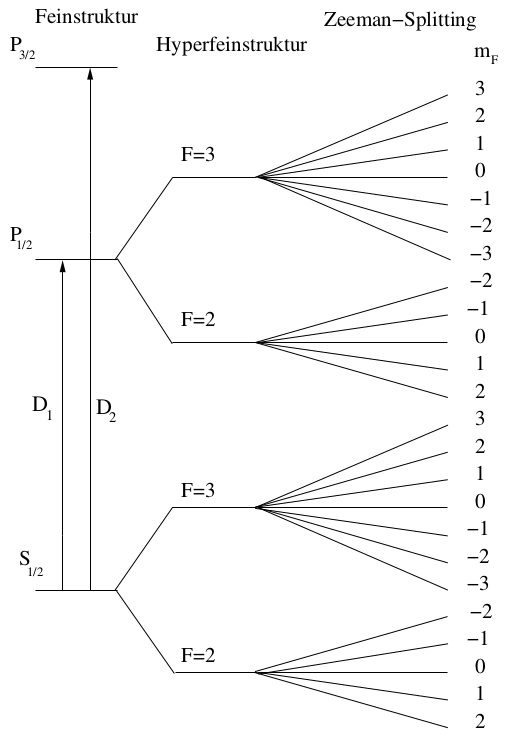
\includegraphics[scale=0.43]{content/schema.png}
    \caption{Die Zeeman-Aufspaltung für  $\ce{^{85}Rb}$ [1]}
    \label{fig:schema}
  \end{figure}

  \begin{figure}[H]
    \centering
    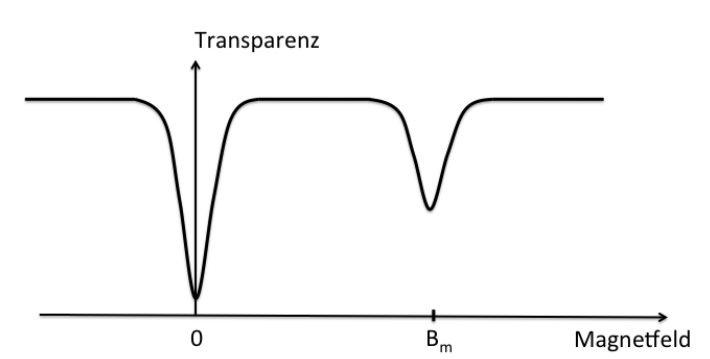
\includegraphics[scale=0.4]{content/bild.png}
    \caption{Tranzparenz eines Rubidiumgases eines Isotopes in Abhängigkeit eines angelegten Magnetfeldes [2]}
    \label{fig:bild}
  \end{figure}


\subsection{Messung der Zeeman-Aufspaltung}

Durch ein variierbares Magnetfeld kann nach Erreichen des gepumpten Zustandes dessen Inversion herbeigeführt werden.
Dies geschieht für ein Magnetfeld

\begin{equation*}
    \label{eqn:lin}
    B_\text{ind.Em.} = \frac{hf}{g_\text{F}\mu_\text{B}} = \frac{4\pi m_\text{e} f}{e g_\text{F}} \; ,
\end{equation*}

welches Photonen erzeugt, die die stimulierte Emission herbeiführen. Diese bewirkt, dass die Transparenz
des Gases für die anregende Strahlung sinkt, wenn eine charakteristische Feldstärke $B_\text{ind.Em.}$ eingestellt wird,
wie in Abbildung \ref{fig:bild} dargestellt.

\subsection{Helmholtzspulen}

Die Feldstärke

\begin{equation}
    B = \mu_0 \frac{8IN}{\sqrt{125}R}
    \label{eqn:helm}
\end{equation}

des homogenen Magnetfeldes eines Helmholtzspurenpaares ist abhängig von der Windungszahl $N$, dem Spulenabstand $R$
und dem durchfließendem Strom $I$.

